% CREATED BY DAVID FRISK, 2016
\chapter{Background}
\label{ch:theory}
%TODO fixa inldning
This chapter will present the theory that will be used in the remainder of the paper. The chapter will be structured as, first notation, theorems, definitions and assumptions  are stated. Then the cryptographic preliminaries used in this paper are explained. In section \ref{sec:RF_theory} two different types of zero knowledge proofs are presented, more precisely range proofs and set membership proofs.

\section{Preliminaries}
This section will introduce some notations and then cryptographic assumptions and definitions followed by several cryptographic preliminaries that will be relevant for this paper. The purpose of this section is to state information that will be refereed to and used as building blocks for the remaining  of this paper.

\subsection*{Notation}
To make the text more comprehensible notation that is used throughout the paper is introduced and defined here.  
%Consider $n$ clients and $m$ servers, to simplify notation define the two sets $\mathcal{N}=\{1,...,n\}$ and $\mathcal{M} = \{1,...,m\}$. Let $c_i$ and $x_i$ for $i\in\mathcal{N}$ denote the clients (data providers) and their respective data. Denote the servers by $s_j$, where $\:j\in\mathcal{M}$.
Let $\mathds{F}=\mathds{Z}_p$ denote a finite field, where $p$ is a large prime and let $\mathds{G}$ denote a unique subgroup of order $q$.  Define $g\in\mathds{G}$ to be a group generator and $h\in\mathds{G}$ a group element, such that  $log_g\:h$ is unknown and $h$ co-prime to $p$. 
The notation $y\in_R\mathds{Y}$, means that an element $y$ in chosen at random from the set $\mathds{Y}$.

\subsection*{Definitions, Theorems and Assumptions}
In this section definitions, theorems and assumption that will be refereed to and used throughout this paper is stated. The assumptions given here are the assumptions that all cryptographic constructions in this paper will rely on. The discrete logarithm assumption and the q-strong Diffie Hellman assumption define below does not hold in the presence of quantum computers. Thus the cryptographic constructions presented in this paper are not  guaranteed to be secure post quantum. 
\vspace{10pt}
\begin{Mydef}[\textbf{Pseudorandom Function (PRF)}]
Let $S$ be a  distribution over $\{0,1\}^l$ and $F_s\: :\: \{0,1\}^m\to\{0,1\}^n$ a family of functions indexed by a string $s$ in the support $S$. It is defined that $\{F_s\}$ is a pseudo random function family if, for every PPT (probabilistic polynomial time) adversary $\mathcal{A}$, there exists a negligable function $\varepsilon$ such that:
\begin{align*}
|\text{Pr}[\mathcal{A}^{F_s}(\cdot) = 1] - \text{Pr}[\mathcal{A}^{R}(\cdot) = 1] | \leq \varepsilon,
\end{align*}
where $s$ is distributed according to $S$ and $R$ is a function sampled uniformly at random from the set of all functions mapping from $\{0,1\}^n$ to $\{0,1\}^m$.
\end{Mydef}
\vspace{10pt}
\begin{Mydef}[\textbf{Euler's totient function}]
The function $\Phi(n)$ is defined as the counter of the number of integers that are relative primes to $n$ in the set $\{1,...,n\}$ . Note if $n$ is a prime number $\phi(n) = n-1$.
\end{Mydef}
\vspace{10pt}
\begin{thm}[\textbf{Euler's Theorem}]
\label{thm:euler}
For all integers $x$ and $n$ that are co-prime it holds that:
$x^{\Phi(n)} = 1\:( \text{mod n})$, where $\Phi(n)$ is Euler's totient function.
\end{thm}
\vspace{10pt}
From Theorem \ref{thm:euler} it follows that for arbitrary $y$ it holds that $x^{y\Phi(n)} = 1 \:( \text{mod n})$.
\vspace{10pt}

\begin{Ass}[\textbf{Discrete logarithmic assumption}]
\label{ass:DLA}
Let $\mathds{G}$ be a group of prime order $q$, further let $g\in \mathds{G}$ be a group generator of $\mathds{G}$ and $y \in\mathds{G}$ be an arbitrary group element. Then it is  infeasible to find $x \in \mathds{Z}_q$, such that $y=g^x$
\end{Ass}

\vspace{10pt}
\begin{Ass}[\textbf{q-strong Diffie Hellman Assumption}]
 Given a group $\mathds{G}$, a random generator $g\in \mathds{G}$ and powers $g^x,...,g^{x_q}$, for $x \in_R \mathds{F}$ and  $q= |\mathds{G}|$. It is then  infeasible for an adversary to find $(c, g^{\frac{1}{x+c}})$, where $c \in \mathds{F}$.
\end{Ass}




\subsection*{Homomorphic Secret Sharing}
Homomorphic secret sharing (HSS), first mentioned in \cite{How_share_A_secret}, hides a secret $x$ by splitting it into shares, such that any subset, $\mathcal{S}$, of shares smaller than a threshold $\tau$, i.e $|\mathcal{S}|<\tau$, reviles no information about the original value of $x$.  Let a secret $x$ be split into $m$ shares denoted $x_i \text{ s.t } i\in\{1,...,m\}$, then to reconstruct the value $x$ at least $\tau$ shares has to be combined, this is called a $(\tau,m)$-threshold scheme. In this paper the threshold will be equal to the number of shares,  $\tau=m$. 

\subsubsection*{Verifiable Additive Homomorphic secret sharing}
In this paper \textit{Verifiable Additive}  homomorphic secret sharing  (VAHSS) will be of interest.  

Before describing VAHSS, AHSS will be desribed. The additivity property for a HSS means that the secret is reconstructed by computing the sum of at least $\tau$ shares, i.e $x = \sum_{i=1}^\tau x_i$. This is denoted Additive Homomorphic Secret Sharing (AHSS).

VAHSS is a construction of AHSS where many parties, refereed to as servers, collaborates to  compute the sum of multiple clients secrets. Each client split their secret into the same amount of shares as there are serves and sends one share to each servers. The servers then computes and outputs a partial sum of all received shares. The final sum is computed by summing the servers outputs. For VAHSS constructions a proof $\sigma$ is constructed that verifies that final sum is the correctly computed sum of the clients secrets. In section \ref{sec:VAHSS-HSS} a specific construction of VAHSS is presented.


\subsection*{Homomorphic hash functions}
Let $\mathcal{H}$ be a cryptographic hash function, $\mathcal{H}:\mathds{F}\mapsto \mathds{G}$. Any such function should satisfy the following two properties:
\begin{itemize}
    \item \textbf{Collision-resistant} It should be hard to find $x,x'\in\mathds{F}$ such that $x\neq x'$ and $\mathcal{H}(x)=\mathcal{H}(x')$.
    \item \textbf{One-Way} It should be computationally hard to find $\mathcal{H}^{-1}(x)$.
\end{itemize}

A homomorphic hash function should also satisfy the following property:
\begin{itemize}
    \item \textbf{Homomorphism} For any $x,x'\in\mathds{F}$ it should hold that $\mathcal{H}(x\circ x') = \mathcal{H}(x)\circ\mathcal{H}(x')$, where $\circ$ is either $"+"$ or $"*"$.
\end{itemize}

A homomorphic hash function that satisfies the thee properties is the function $\mathcal{H}_1(x):\mathds{F}\mapsto\mathds{G}$ and $\mathcal{H}_1(x)= g^{x}$ \cite{HHF}. 



\subsection*{Pedersen Commitment scheme}
A \textit{Pedersen commitment} is a commitment to a secret $x\in\mathds{F}$, defined as $\mathds{E}(x,R)=g^xh^R$, where $R\in_R\mathds{F}$, \cite{pedersen}. The Pedersen commitment satisfies the following theorem:
\\
\begin{thm}
\label{thm:C=g^xh^R}
For any $x\in\mathds{F}$ and for $R\in_R\mathds{F}$, it follows that   $\mathds{E}(x,R)$ is uniformly distributed in $\mathds{G}$. If two commits satisfys $\mathds{E}(x,R)=\mathds{E}(x',R')$  $x\neq x'$ then it must hold that $R\neq R' \:\text{mod}\:q$ and 
\begin{equation}
\label{eq:pedersen_binidng}
   x-x' =  (R-R')\:log_g\:h \text{ mod }p \quad \text{Where p is the prime underlying the field }\mathds{F} .
\end{equation}
\end{thm}
\begin{proof}
The statements of the theorem follows from solving for $log_g(h)$ in $\mathds{E}(x,R)=\mathds{E}(x',R')$ 
\end{proof}

Theorem \ref{thm:C=g^xh^R} implies that if someone knows the discrete logarithm of $h$ with respect to $g$, i.e $log_g(h)$, this person is able to provide two equal commits, $\mathds{E}(x,R)=\mathds{E}(x',R')$ such that $x\neq x'$. Since the $log_g h$ is assumed to be unknown it is impossible to construct two equal commits hiding different secrets. This means that the Pedersen commitment scheme is computational binding under the discrete logarithm assumption, it is also perfectly hiding of the secret $x$, \cite{pedersen}. 

The Pedersen commitment is homomorphic. Hence for arbitrary messages $x_1,x_2\in\mathds{F}$, random values $R_1,R_2\in_R\mathds{F}$ and the commits $C_i=\mathds{E}(x_i,R_i),\:i\in\{1,2\}$, it holds that $C_1\cdot C_2 = \mathds{E}(x_1+x_2,R_1+R_2)$.

Note that the Pedersen commitment is similar to the hash function $\mathcal{H}_1$ and the hash function can be seen as a generalisation of the Pedersen commitment.

A Pedersen commitment scheme can also be defined for vectors and is then called \textit{Pedersen vector commitment}. Consider a $n$ dimensional vector $\mathbf{x}\in\mathds{F}^n$, let $\mathbf{g}=(g_1,...,g_n) \in\mathds{G}^n$ and $h\in\mathds{G}$ where $\mathds{G}$ is a group of order $q$ as above. A commitment to the vector  $\mathbf{x}=(x_1,...,x_n)$  with the random value $R\in_R \mathds{F}$ is then defined as $\mathds{E}(\mathbf{x},R) = \mathbf{g}^\mathbf{x}h^R = h^R\prod_{i=1}^n g_i^{x_i}$ and the commitment is a value in the one-dimensional group $\mathds{G}$. 

\subsection*{Bilinear mapping}
\label{sec:bilinear}
Bilinear mapping (also commonly called bilinear pairing) maps two group elements from one groups to an element in another group. In this paper admissible bilinear mapping fulfilling Definition \ref{def:AdmissibleBM} will be used. In the definition given here two elements from the same group are mapped.  Generally in the definition of admissible bilinear mapping,  two elements from different groups are mapped to a third group, i.e $e: \: \mathds{G}_1\times \mathds{G}_2 \to \mathds{G}_T$, but in this paper it will always hold that $\mathds{G}_1=\mathds{G}_2$ and hence the definition is given on this form. 
\begin{Mydef}[\textbf{Admissible Bilinear Map}]
	\label{def:AdmissibleBM}
	Let $\mathds{G}_1,\mathds{G}_T$ be two multiplicative cyclic groups of prime order $p$ such that there exist an admissible bilinear map $e: \: \mathds{G}_1\times \mathds{G}_1 \to \mathds{G}_T$. Let $\mathds{G}_1^*=\mathds{G}_1\backslash \{1\}$.  Then the bilinear map $e$ fulfils:
	\begin{itemize}
		\item Bilinear: for any group element  $g\in\mathds{G}_1^*$ and $a,b \in \mathds{Z}_p$,
		\begin{align*}
			e(g^a,g^b) = e(g,g)^{ab}
		\end{align*}	
		\item Non-degenerated: $e(g,g)\neq 1$	 
		\item The bilinear map is efficiently computable
	\end{itemize}
\end{Mydef}

\subsection*{Bohen-Boyen Signatures}
Considering a bilinear map $e$, defined in the previous section. The bilinear property of the mapping $e$ can be used to create digital signatures. Bohen-Boyen presented a signature scheme that exploits the bilinear property of the mapping $e$ to verify signatures \cite{Bohen-Boyen}.  In short the scheme works as, the signer knows the secret key $x$ and distributes the public key $g^x$. To sign a message $m$ the signer uses the secret key, $x$, and computes $\sigma = g^{1/(x+m)}$. This signature is $q-secure$ to forgery under the q-Strong Diffie Hellman Assumption. Verification is done by checking that $e(\sigma,y\cdot g^m) = e(g,g)$, which holds due to the bilinearity of $e$. 


\subsection*{Zero knowledge proof}
Zero-knowledge proofs (ZKP) is a cryptographic primitive that was first presented in \cite{OG_ZKP}. The idea behind a ZKP is that after successfully performing a ZKP a certain statement about a secret $x$ has been verified to be true (or false) without having revealed any other information about the secret $x$ beyond the statement. Here only non-interactive ZKP that ensures proof of knowledge (PoK) is considered.  Before closer defining what this means the set up and environment of ZKP protocols is defined

A ZKP consists of two parties a \textit{prover} and a \textit{verifier}, further assume both parties has access to the protocol parameters generated by a SetUp algorithm and a language $\mathcal{L}\in \text{ NP}$, additionally the prover knows a secret $x\in \mathcal{L}$. The prover constructs a proof that $x$ belongs to $\mathcal{L}$, by using a witness $w$ of $x$. Given the proof the verifier can in polynomial time determine if the proof is valid or not. 
For a ZKP to be non-interactive means that there is no communication required between the prover and verifier during the construction of the proof. PoK means that the verifier is not only convinced there exist a witness $w$ but also that the prover knows such a witness.

 A ZKP should fulfil the thee properties in Definition \ref{def:ZKP}, informally the definitions states that: a correctly constructed proof of an instance $x\in\mathcal{L}$ should be accepted with probability $1$, an incorrect proof of an instance $x\notin\mathcal{L}$ should have a negligible probability of being accepted and the verifier should learn nothing about the secret beyond the statement being proved.
 

\begin{Mydef}
\label{def:ZKP}
First define the two algorithms;  \texttt{Prove}$(x,w)$,the algorithm for generating a ZKP of instance $x\in\mathcal{L}$ and witness $w$, and  \texttt{Verify}, the verification algorithm of the ZKP. Such a ZKP scheme  should fulfil the three properties: 
\begin{itemize}
\item \textbf{Completeness} Given a witness $w$ satisfying the instance $x\in\mathcal{L}$, it should hold that \texttt{Verify}$($\texttt{Prove}$(x,w)) = 1$. 
\item \textbf{Soundness} If the witness $w$ does not satisfy the  instance $x\notin\mathcal{L}$, then the probability  Prob$[$\texttt{Verify}$($\texttt{Prove}$(x,w)) = 1] < \varepsilon$, for a sufficiently small $\varepsilon$. 
\item  \textbf{Zero-knowledge} A proof system is \textit{honest verifier zero-knowledge} if there exist a PPT algorithm \texttt{Simulator} having access to the same input as the algorithm \texttt{Verify} but not the provers input, such that output from the \textt{Simulator} and \texttt{Prove} is indistinguishable, i.e have the same distribution given that $x\in\mathcal{L}$.  
\end{itemize}
\end{Mydef}
 
This paper will consider zero knowledge range proof (ZKRP) and zero knowledge set membership proofs (ZKSM) where the statement that the prover convinces the verifier of is that the secret belongs to a predetermined range or set.


\subsection*{Fiat-Shamir heuristic}
The Fiat-Shamir heuristic \cite{Fiat-Shamir} can be used to convert an interactive protocol into a non-interactive. In this paper it will be used to construct non-interactive ZKP. A non interactive  ZKP requires no communication between the prover and verifier during the construction of the proof. In interactive constructions the verifier sends a challenge $c\in_R\mathds{F}$ to the prover that is included in the proof in order to convince the verifier that the prover did not cheat. The Fiat-Shamir heuristic replaces the random challenge sent by the verifier with the output of a hash-function of the partial-proof up to this point. The Fiat-Shamir heuristic converts an interactive ZKP to non-interactive while preserving security and full zero-knowledge relying on the random oracle model (ROM) \cite{Fiat-Shamir} .




%%%%%%%%%%%%%%%%%%%%%%%%%%%%%%%%%%%%%%%%%%%%%%%%%%%%%%
%%%%%%%%%%%%%%%%%%%%%%%%%%%%%%%%%%%%%%%%%%%%%%%%%%%%%%
%%%%%%%%%%%%%%%%RANGE%%%%PROOF%%%%%%%%%%%%%%%%
%%%%%%%%%%%%%%%%%%%%%%%%%%%%%%%%%%%%%%%%%%%%%%%%%%%%%%
%%%%%%%%%%%%%%%%%%%%%%%%%%%%%%%%%%%%%%%%%%%%%%%%%%%%%%
\section{Set Membership Proof and Range Proofs}
\label{sec:RF_theory}

Zero knowledge set memberships proof (ZKSM)  allows a prover to convince a verifier that the value of a secret is in an allowed set.  Zero knowledge set membership proofs (ZKSM) does this without revealing any other information about the secret beyond the fact that the secret belongs to the set. Formally  (ZKSM) prove the following statement:
\begin{align} \label{eq:SM_statement}
    \{(g,h\in\mathds{G},C;x,R\in\mathds{F})\::\:C= g^x h^R \wedge x \in \Phi\},
\end{align}
where $\Phi$ is some known set. 
 
Zero knowledge range proofs (ZKRP) will also be considered, they prove that a secret belongs to a range, instead of a set, which is not as general as a set since it has to be continuous.  Zero knowledge range proofs (ZKRP) does not revealing any other information about the secret beyond the fact that the secret belongs to the range. Formally the ZKRP presented in this paper are constructed to prove the following statement about a secret $x$:
\begin{align} \label{eq:RP_statement}
    \{(g,h\in\mathds{G},C;x,R\in\mathds{F})\::\:C= g^x h^R \wedge x \in \{\textit{"predetermined allowed range"}\}.
\end{align}
The range which $x$ is proved to belong to in ZKRPs may vary between different constructions and will be more precisely defined below for the separate constructions. 

Note that in the above statements  it is assumed that $x$ is the secret hidden in a Pedersen commitment, which is not a general requirement for range proofs and set membership proofs however only such proofs will be studied in this paper. 

All set membership proofs and range proofs considered in this paper satisfied Definition \ref{def:ZKP}.

%Let $\mathcal{P}$ rand  $\mathcal{V}$ denote the two parties prover respectively verifier, an informal explanation the statements in equations \eqref{eq:RP_statement}, \eqref{eq:SM_statement} is: after successfully performing a range proof  $\mathcal{P}$ has convinced $\mathcal{V}$, that the secret $x$ in a Pedersen commitment $C$ is in an predetermined allowed range (or set) without $\mathcal{V}$ learning anything else about $x$.

%There exists several constructions for range proofs and set membership proofs however this paper will investigate two different range proof constructions and one set membership construction. These constructions will then in the next chapter be investigated if they can be combined with the VAHSS-construction described above to ensure clients honesty in the  VHASS construction.

% Before presenting these two a XXX will be given to motivate the choice of these two ZKRP. (TODO )Square based range proofs \cite{Efficient_proof_interval} %what is is and why do not use. 
%Another construction which could be used to construct a prove that a value is in an allowed range is function secret sharing \cite{FSS} % explain what and why not use.

%In the two subsections below the theory and construction of \textit{Set membership proofs \& Signature based range proofs}  and \textit{Bulletproofs} are presented. All proofs satisfies the three conditions \textit{completeness}, \textit{soundness} and \textit{zero-knowledge} stated in Definition \ref{def:ZKP} and proves a statement on the form given in equation \eqref{eq:RP_statement} or \eqref{eq:SM_statement}.

%\subsection{Square based}
%\cite{Effifient_proof_interval} Based on strong RSA-assumption --> not strong any more removed by %\cite{remove_strong_RSA}

%$\mathds{Z}_n, n=p\cdot q$

%The Fujisaki-Okamoto Commitment Scheme differense from pedersen? 

\subsection*{Signature-based  Set membership proof and range proof}
In this section a specific implementation of a ZKSM is described. It will then be explained how this ZKSM can be extended to a ZKRP. The set membership proof described in this section will be refereed to as \textit{signature based set membership} and the derived range proof will be refereed to as \textit{signature based range proof}. Both the set membership proof and the derived range proof was originally presented in \cite{RANGE-SET}. Both the proofs  are modified compared to the original construction according to the Fiat-Shamir heuristic to be non-interactive.

\subsubsection*{Set membership proof}
The idea behind the ZKSM is that for each element in the allowed set $\Phi$ there exist a public commitments, denoted $A_i, \: \forall i\in\Phi$.  These commitments are made public in the SetUp phase by the verifier or some other party (not the prover). The prover aims to prove that the secret hidden by a pre-published Pedersen commitment, denoted $C$, is in the allowed set $\Phi$. To prove this the public commitment representing the secret $x$, i.e $A_x$  is selected and  used to compute the value $V = A_x^\tau$, where $\tau\in_R\mathds{F}$. The prover has to convince the verifier that  1) the published value $V$ is indeed equal to  $A_x^\tau$ where $A_x$ is a signature of an element from the allowed set  2) the secret in the Pedersen commitment $C$  is the same as the secret hidden by $V$.
%The first two constructions that will be considered here are based on the range proofs presented in \cite{RANGE-SET} and adjusted to a non-interactive construction described by \cite{ZKRP_Morais}. The transformation from a interactive protocol to a non interactive is done via the Fiat-Schit principle \cite{fiat-schmit}.  Non-interactive means that there communication between the prover and verifies while XXX Find. 
%Construction \ref{alg:ZKSM} is a non interactive set membership proof of a Pedersen commitment $C=g^\sigma h^R$, where $\sigma$ is the secret and $R\in_R\mathds{F}$ is chosen uniformly at random.
%The construction allows a prover, that knows the secret $x$, to convince the verifier, who has access to the commitment $C$, that $x\in\Phi$ for some predetermined set $\Phi$ without revealing any other information regarding the secret $x$.  

In Construction \ref{alg:ZKSM} a detailed description of the  PPT algorithms constructing  the ZKSM described above is explained. The notation $e(\cdot,\cdot)$ in the construction refers to an admissible bilinear mapping as defined previously in section \ref{sec:bilinear}.
%This construction fulfils the zero knowledge requirements described in \ref{sec:ZK} and is a non interactive zero knowledge set membership proof. 
\begin{algorithm}[]
\caption{\textbf{: Non interactive set membership proof}}
\textbf{Goal:} Given a Pedersen commitment $C=g^x h^R$ and a set $\Phi$, prove that the secret $x$ in the commitment belongs to the set $\Phi$ without revealing anything else about $x$.
\vspace{2pt} \hline \vspace{2pt}
\begin{itemize}
  \item\textbf{SetUp $(1^{\lambda}, \Phi)\xrightarrow[]{}(sk,pp)$}\\
Pick uniformly at random $\chi\in_R\mathds{F}$ and put the secret key $sk=\chi$. Define $y=g^\chi$ and $A_i=g^{\frac{1}{\chi+i}} \:\forall i\in\Phi$, output $y$ and $\{A_i\}_{i\in\Phi }$ and define the public parameters $pp=(y,\{A_i\}_{i\in\Phi})$.

\item\text{\textbf{Prove} $(g,h,C,\Phi)\xrightarrow[]{}\Sigma=(V,a,D,z_x,z_\tau,z_R)$}\\
Pick uniformly at random $\tau\in_R\mathds{F}$, choose from the set $\{A_i\}$ the element $A_x$ and calculate $V=A_x^\tau$. Pick uniformly random three values $s,t,m\in_R\mathds{F}$. Put $a=e(V,g)^{-s}e(g,g)^t$ and $D=g^sh^m$. Then use these two values to compute the challenge $c=\text{Hash}(C,V,a,D)$. Then given this challenge compute $z_x = s-x c$, $z_R = m-Rc$ and $z_\tau= t-\tau c$ then construct and publish the proof, $\Sigma = (V,a,D,z_x,z_\tau,z_R)$.

\item\text{\textbf{Verify} $(g,h,C,\Sigma)\xrightarrow[]{}\{0,1\}$}\\
Check if $D\overset{?}{=}C^ch^{z_R}g^{z_x}\wedge a \overset{?}{=} e(V,y)^c e(V,g)^{-z_x}e(g,g)^{z_\tau}$. If the equality holds the prover has convinced the verifier that the secret $x\in\Phi$ thus return $1$ otherwise return $0$.
\end{itemize}
\label{alg:ZKSM}
\end{algorithm}

The ZKSM construction can be turned into a efficient zero knowledge range proof by rewriting the secret $x$ in base $u$ such that,
\begin{align*}
    x = \sum_{j=0}^{l-1} x_ju^j.
\end{align*}
Using this notation it follows that if $x_j\in[0,u)\: \forall j\in\mathds{Z}_l$, then $x\in[0,u^l)$. A remark is that the subscript $j$ goes between the number $[0,l-1]$ and not $[0,l]$.
 %This has been wrongly notated \cite{RANGE-SET,ZKRP_Morais} and therefore an explicit proof of this is given in Appendix \ref{appendix:range}. 
% Construction \ref{alg:ZKRP} is a modification of construction \ref{alg:ZKSM} into a non interactive zero knowledge range proof using the above decomposition of the secret $x$.
\begin{comment}
\begin{algorithm}[]
\caption{\textbf{: Non interactive range proof}}
\textbf{Goal:} Given a Pedersen commitment $C=g^x h^R$ and two parameters $u,l$, prove that the secret $x=\sum_{j=0}^l x_j u^j$ belongs to the interval $[0,u^l)$ without revealing anything else about $x$.
\vspace{2pt}
\hline
\vspace{2pt}
\begin{itemize}
  \item\textbf{SetUp $(g,h,u,l)\xrightarrow[]{}(y,\{A_{i}\}_{i\in\mathds{Z}_u})$}\\
Pick uniformly at random $\chi\in_R\mathds{F}$. Define $y=g^\chi$ and $A_i=g^{\frac{1}{\chi+i}} \: \forall i\in\mathds{Z}_u$, output $y$ and $\{A_i\}$.

\item\text{\textbf{Prove} $(g,h,C,u,l)\xrightarrow[]{}\textit{ proof}_{RP}=(\{V_j\},\{a_j\},D,\{z_{x_j}\},\{z_{\tau_j}\},z_R)$}\\
 For every $j\in\mathds{Z}_l$: pick uniformly at random $\tau_j\in_R\mathds{F}$ and compute $V_j=A_{x_j}^{\tau_j}$. Then pick uniformly at random three more values $s_j,t_j,m_j\in_R\mathds{F}$ and compute $a_j=e(V_j,g)^{-s_j}e(g,g)^{t_j}$ for all $j\in\mathds{Z}_l$ and $D=\prod_{j\in\mathds{Z}_l}(g^{u^js_j})h^{m_j}$ Given this let $c=\text{Hash}(C,\{V_j\}\{a_j\},D)$. Then for all $j\in\mathds{Z}_l$ compute $z_{x_j}=s_j-x_jc$,$z_{\tau_j}=t_j-\tau_jc$ and $z_R=m-Rc$, where $m=\sum_{j\in\mathds{Z}_l}m_j$. Finally output the proof: \textit{proof}$_{RP}=(\{V_j\},\{a_j\},D,\{z_{x_j}\},\{z_{\tau_j}\},z_R)$ 

\item\text{\textbf{Verify} $(g,h,C,\textit{proof})\xrightarrow[]{}\{0,1\}$}\\
Check if $D\overset{?}{=}C^ch^{z_R}\prod_{j\in\mathds{Z}_l}(g^{u^j z_{x_j}})\wedge a_j \overset{?}{=} e(V_j,y)^c e(V_j,g)^{-z_{x_j}}e(g,g)^{z_{\tau_j}}$ for all $j\in\mathds{Z}_l$.  If the equality holds the prover has convinced the verifier that $x\in [0,u^l)$ return $1$ otherwise return $0$.
\end{itemize}
\label{alg:ZKRP}
\end{algorithm}
\end{comment}
This ZKRP construction can be generalised to  prove membership to an arbitrary interval $[a,b]$ where $a>0$ and  $\:b>a$, by showing  that $x\in[a,a+u^l)$ and $x\in[b-u^l,b)$, since then the secret belong to the range $[a,b]$. Figure \ref{fig:interval} illustrates the intuition and correctness of the statement.  Proving $x\in[a,a+u^l)$ and $x\in[b-u^l,b)$ can easily be transferred into proving $x-a\in[0,u^l)$ and $x-b+u^l\in[0,u^l)$, since both $a,b$ are public. 
%Therefore to prove a secret is in an arbitrary interval the steps \textbf{Prove} and \textbf{Verify} for a signature based range proof will have to be executed twice. Plus the  \textbf{Verify} algorithm has to be modified to include an \texttt{AND} operation to verify that  $x-a\in[0,u^l) \wedge x-b+u^l\in[0,u^l)$.
 In \cite{arbitary_range_opt} an optimised implementation of the arbitrary range signature based range proof is presented, reducing the complexity with a factor $2$. This rather small reduction is important when a verifier is required to check the range of multiple secret simultaneously.

\begin{figure}[]
    \centering
    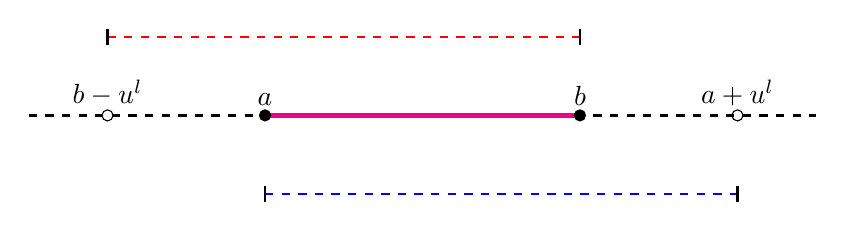
\begin{tikzpicture}
        \draw[dashed, blue, thick] (-2,0) -- (4,0);
        \draw[black, thick] (-2,-0.1) -- (-2,0.1);
        \draw[black, thick] (4,-0.1) -- (4,0.1);
        
        \draw[dashed, black, thick] (-5,1) -- (5,1);
        \draw[magenta, ultra thick] (-2,1) -- (2,1);
 
        
        \draw[dashed, red, thick] (-4,2) -- (2,2);
        
        \draw[black, thick] (-4,1.9) -- (-4,2.1);
        \draw[black, thick] (2,1.9) -- (2,2.1);
        
          
        \draw [black] (-4,1) circle (2pt) node[anchor=south] {$b-u^l$};

        \filldraw [black] (-2,1) circle (2pt) node[anchor=south] {$a$};

        \filldraw [black] (2,1) circle (2pt) node[anchor=south] {$b$};

        \draw [black] (4,1) circle (2pt) node[anchor=south] {$a+u^l$};
    \end{tikzpicture}
    \caption{Illustration of generalisation to arbitrary intervals $[a,b]$ for range proofs}
    \label{fig:interval}
\end{figure}


%TODO fix 
\subsection*{Bulletproofs}
Bulletproofs is a state of the art range proof that is integrated in many real-world protocols,  for example they are often used in in cryptocurrencies. Bulletproof will be used in this paper for runtime comparison to an state of the art construction.  
%TODO longer here

The Bulletproof was originally presented in \cite{bulletProofs_theory}. Bulletproof are range proofs that a secret belongs to the range $[0,2^n]$,m and are of logarithmic in $n$ in size. The Bulletproof construction is based on the inner product argument. The inner product argument is an argument of knowledge that $\textbf{s},\mathbf{q}$ in a Pedersen vector commitment $P_v=\mathbf{g}^\mathbf{s}\mathbf{h}^\mathbf{q}$ satisfies a given inner product denoted $c$. 

%In appendix \ref{appendix:BP} a more precise definition of Bulletproofs is given. Construction \ref{alg:bullet} in appendix \ref{appendix:BP} the bulletproof construction modified compared to \cite{bulletProofs_theory} to be non-interacitve using the Fiat-Shamir heuristic.
%mention vector commitment, inner product and logarithm n , describe runtime. Fia shamir

% logarithmic in the size of the range that builds on the inner product argument presented below. which allows a prove to convince a verifier that he knows the opening $\bm{s},\bm{q}\in\mathds{F}^n$ to a Pedersen vector commitment $P_v = \bm{g}^{\bm{s}}\bm{h}^{\bm{q}}$ such that the inner product of $\bm{s},\bm{q}$ is equal to a known value, $c$. This can be done with a proof of size $log\: n$, compare to the trivial solution of publishing $\bm{s},\bm{q}$ which is a proof of size $n$.

%\subsubsection*{Notation and Set Up}
%Before describing the construction of Bulletproofs, some additional notation is introduces.  Note that here the same notation  that is used in original Bulletproof paper, will be used, hence more details of the notations can bee seen in \cite{bulletProofs_theory} . 


% and will not be redefined instead the reader is encurraged to .  which will be presented here. First let lowercase bold font variables denote vectors, i.e $\mathbf{a}\in\mathds{F}^n$ is a vector with element $a_1,..,a_n \in \mathds{F}$, and uppercase bold font variables denote matrices, i.e $\mathbf{A}\in\mathds{F}^{n\times m}$ is a matrix and $a_{ij}$ the element of $\mathbf{A}$ at row $i$ and column $j$. Given this notation denote scalar multiplication with a vector as $\mathbf{b}=c\cdot \mathbf{a}\in\mathds{F}^n$, where $c\in\mathds{F}$ and  $b_i=c\cdot a_i, \: i\in\{1,...,n\}$. Denote the euclidean inner product of two vectors as $\langle \mathbf{a},\mathbf{b}\rangle$ and Hadamard product as $\mathbf{a}\circ \mathbf{b}$.

%Further consider vector polynomials $p(X)$ of degree $d$ on the form $p(X)=\sum_{i=0}^d \mathbf{p_i}\cdot X^i\in\mathds{F}^n[X]$, where the coefficients $\mathbf{p_i}\in\mathds{F}^n$. The inner product of two vector polynomials, $l(X),r(X)$ is defined as, 
%\begin{align*}
  %  \langle l(X),r(X)\rangle = \sum_{i=0}^d\sum_{j=0}^n \langle l_i,r_j\rangle \cdot X^{i+j}\in\mathds{F}[X].
%\end{align*}
%The following is equivalent: evaluating two polynomials at $x$ then taking the inner product versus taking the inner product polynomial at $x$.

%Let $\mathbf{a}||\mathbf{b}$ denote the concatenation of two vectors. Python notation will be used to denote sections of vectors such that $\mathbf{a}_{[:l]} = (a_1,...,a_l)$ and $\mathbf{a}_{[l:]} = (a_{l+1},...,a_n)$ for $l\in[1,n]$. 

%For $k\in\mathds{F}^*$ let $\mathbf{k}^n=(1,k,k^2,...,k^{n-1})$, i.e the vector containing the $n$ fist powers of $k$. 

%Let $\mathbf{g},\mathbf{h}\in\mathds{G}^n$ and remember that $\mathbf{a}\in\mathds{F}^n$ then define $C= \mathbf{g}^\mathbf{a} = \prod_{i=1}^ng_i^{a_i}\in\mathds{G}$, where $C$ can be interpreted as a commitment to the vector $\mathbf{a}$. In this section the two vectors $\mathbf{g},\mathbf{h}$ will be considered to be generators of the space $\mathds{G}^n$.

%In this section $n$ will denote the dimension of the room not the number of clients as earlier. Further remark that, the dimension of the room is the length of the bit representation of the secret in the Pedersen vector commitment, potentially padded with zeros.

%Both in the construction of the inner product argument and the Bulletproof the parameters $g,h,\mathbf{g},\mathbf{h},u$ are assumed to be pre-shared and known by both verifier and prover. The group elements $g,h$ are as before. Further the two vectors $\mathbf{g}, \mathbf{h} \in \mathds{G}^n$ are assumed to be independent generators of the space $\mathds{G}^n$. The variable $u\in\mathds{G}$ is such that there is no known discrete logarithmic relation between $\mathbf{g},\mathbf{h}$. In order to ensure the fairness and correctness of the parameters $g,h,\mathbf{g},\mathbf{h},u$ they can be  assumed to be chosen by some trusted third party. Another possibility that drops the assumption of a trusted setup is to use the \textit{Nothing Up My Sleeve} (NUMS) strategy, \cite{ZKRP_Morais}.

%\subsubsection*{Inner product argument}
%\label{sec:inner_prod}
%The Bulletproof construction is based on the inner product argument which will be closer presented in this section. The inner product argument is an argument of knowledge that $\textbf{s},\mathbf{q}$ in a Pedersen vector commitment $P_v=\mathbf{g}^\mathbf{s}\mathbf{h}^\mathbf{q}$ satisfies a given inner product denoted $c$. 
%(To differ from the Pedersen vector commitment considered here and the Pedersen commitment in the range proofs the exponents in the commit are denoted $\mathbf{s},\mathbf{r}$ instead of $\sigma,R$, and the commitment by $P_v$) 
%More formally the argument is a proof of the statement,
%\begin{align*}
 %   \{(\mathbf{g},\mathbf{h}\in\mathds{G}^n,\:P_v\in\mathds{G},\:c\in\mathds{F};\: \mathbf{s},\mathbf{q}\in\mathds{F}^n) : \: P_v=\mathbf{g}^\mathbf{s}\mathbf{h}^\mathbf{q}\wedge\: c =\langle\mathbf{s},\mathbf{q}\rangle\}
%\end{align*}
%Which can be shown to be equivalent to a proof of the statement,
%\begin{align*}
 %   \{(\mathbf{g},\mathbf{h}\in\mathds{G}^n,\: u,P_v\in\mathds{G};\: \mathbf{s},\mathbf{q}\in\mathds{F}^n) : \: P_v=\mathbf{g}^\mathbf{s}\mathbf{h}^\mathbf{q}u^{\langle\mathbf{s},\mathbf{q}\rangle}\}.
%\end{align*}

%A logarithmic sized proof of the above inner product statement is presented in Construction \ref{alg:inner_product} in Appendix \ref{App:innerP}. The presented  construction is modified compared to the one presented in \cite{bulletProofs_theory} to be non-interactive using the Fiat-Shamir heuristic.

\begin{comment}
\begin{algorithm}
\caption{\textbf{: Inner-product argument}}
\textbf{Goal:} Given a Pedersen vector  commitment $P_v=\bm{g}^{\bm{s}} \bm{h}^{\bm{q}}$ and a value $c$ prove that the two vectors $\bm{s},\bm{q}$ satisfies $\langle\bm{s},\bm{q}\rangle=c$.
\vspace{2pt}
\hline
\vspace{2pt}
\begin{itemize}
\item\text{\textbf{Prove} $(\mathbf{g},\mathbf{h},u,P_v,c,\mathbf{s},\mathbf{q})\xrightarrow[]{}\textit{proof}_{IP}$}\\
Let $y=\text{Hash}_{IP}(\mathbf{g},\mathbf{h},P_v,c) \in\mathds{F}^*$ and compute $P_v'= u^{y\cdot c}P$. Let $\mathbf{l},\mathbf{r}$ be two empty vectors. Run the recursive algorithm \textbf{GenerateProof}$(\mathbf{g},\mathbf{h},u^{x\cdot c},P_v,c,\mathbf{s},\mathbf{q},\mathbf{l},\mathbf{r})$ use the output $(g',h',u',P_v',s',q',\mathbf{l},\mathbf{r})$ to construct the inner product proof $\text{proof}_{IP} =(\mathbf{g},\mathbf{h},u',P_v,s',q',\mathbf{l},\mathbf{r} )$ and output $\textit{proof}_{IP}$. 
\item\text{\textbf{GenerateProof}$(\mathbf{g},\mathbf{h},u,P_v,\mathbf{s},\mathbf{q},\mathbf{l},\mathbf{r}) \xrightarrow[]{}  (g,h,u,P_v,s,q,\mathbf{l},\mathbf{r})$}
\begin{itemize}
    \item If the dimension of the vectors $\mathbf{g},\mathbf{h},\mathbf{s},\mathbf{q}$  drop the bold font and publish the proof $\textit{ proof}_{IP}=(g,h,P_v,u,s,q,\mathbf{l},\mathbf{r})$.
    \item  Otherwise:  Let $n'=n/2$ and define  $c_L=\langle \bm{s}_{[:,n']},\bm{q}_{[n',:]} \rangle$ and $c_R=\langle \mathbf{s}_{[n',:]},\mathbf{q}_{[:,n']} \rangle$. Then use these variables to calculate $L=\mathbf{g}_{[n':]}^{\mathbf{s}_{[:n']}} \mathbf{h}_{[:n']}^{\mathbf{q}_{[n':]}} u^{c_L}$ and $R=\mathbf{g}_{[:n']}^{\mathbf{s}_{[n':]}} \mathbf{h}_{[n':]}^{\mathbf{q}_{[:n']}} u^{c_R}$. Append  $L,R\in\mathds{G}$ to the vectors $\mathbf{l}$ resp $\mathbf{r}$. Now update $y=\text{Hash}_{BP}(L,R)$, and update $\mathbf{g}' = \mathbf{g}_{[:n']}^{y^{-1}}\mathbf{g}_{[n':]}^{y}$, $\mathbf{h}' = \mathbf{h}_{[:n']}^{y}\mathbf{h}_{[n':]}^{y^{-1}}$ and the commitment $P_v'=L^{y^2}PR^{y^{-2}}$. Finally update the vectors $\mathbf{s},\mathbf{q}$ to $\mathbf{s}' = \mathbf{s}_{[:n']}y+\mathbf{s}_{[n':]}y^{-1}$ and $\mathbf{q}' = \mathbf{q}_{[:n']}y^{-1}+\mathbf{q}_{[n':]}y$. Run the algorithm recursively, \textbf{GenerateProof}$(\mathbf{g}',\mathbf{h}',u,P_v',\mathbf{s}',\mathbf{q}',\mathbf{l},\mathbf{r})$ with the updated variables. Note that the vectors $\mathbf{g},\mathbf{h},\mathbf{s},\mathbf{q}$ now have the dimension $n'=n/2$, hence performing the recursion until one-dimensional vectors will require $log\:n$ iterations.
\end{itemize}
\item\text{\textbf{Verify} $(\textit{proof}_{IP} = (\mathbf{g},\mathbf{h},u,P_v,s,q,\mathbf{l},\mathbf{r}))\xrightarrow[]{}\{0,1\}$}\\
For $i\in\{0,log(n)\}$ put $n=n/2$ and $y=\text{Hash}(\bm{l}[i],\bm{r}[i])$, then update the vectors $\bm{g}$ and $\bm{h}$ as well as the  variable $P_v'$ according to, $\bm{g}'= \bm{g}_{[:,n]}^{y^{-1}} \bm{g}_{[n,:]}^{'y}$, $\bm{h}= \bm{h}_l{[:,n]}^{x}\bm{h}_{[n,:]}^{y^{-1}}$ and $ P_v' = L^{y^2}PR^{y^{-2}}  $. After iterating over all $i$ the dimension of the vectors $\bm{g},\bm{h}$ is one and the bold font can be dropped. Compute  $c=\langle s, q\rangle$ and  accept if $P_v' =g^sh^ru^c$.
\end{itemize}
\label{alg:inner_product}
\end{algorithm}
\end{comment}


%The setup phase of construction \ref{alg:inner_product} is intently left out since to avoid a trusted third party a \textit{Nothing up my sleeve} strategy will be used and is described separately in  section \ref{sec:NOMS}.
 

%\subsubsection*{Bulletproofs construction}
The basic idea behind the construction of Bulletproofs is that a prover, given a Pedersen commitment $C=g^x h^R$, of the secret $x$, convince a verifier that the secret belongs to the interval $[0,2^n)$. This is achieved by convincing the verifier that  $\bm{x}\in\{0,1\}^n$ is the binary representation of the secret $x$, or equivalently that $x= \langle \bm{x},\mathbf{2}^n\rangle $ and that the prover knows $\bm{x}$. 

In this paper Bulletproof modified, compared to the original construction given in \cite{bulletProofs_theory}, according to the Fiat-Shamir heuristic to a non-interactive implementation is considered.  A complete description of the construction of a non interactive Bulletproof is given in Appendix \ref{Appendix:Bulletproof} in Construction \ref{alg:bullet}. A non-interactive construction of the inner product argument is given in Construction \ref{alg:inner_product}. 
   % \item $\bm{\bar{x}}$ is the component-wise complement of $\bm{x}$. This is equivalent to show that $\bm{\bar{x}}$ satisfies the two conditions: $\bm{\bar{x}}\circ \bm{x}=\bm{0}^n$ and $\bm{\bar{x}} = \bm{x} -\bm{1}^n \: \text{mod }2$.
%\end{itemize}
%This can be shown to be done by proving the following statement;
%\begin{align}
 %   \big\langle \bm{x} -z\cdot \bm{1}^n, \bm{y}^n\circ (\bm{\bar{x}} + z \cdot\bm{1}^n) + z^2\cdot\bm{2}^n \big\rangle = z^2\cdot x+ \delta(y,z),
%    \label{eq:range_non_zero}
%\end{align}
%where $\bar{\bm{x}}$ is the component-wise complement of $\bm{x}$ and $\delta(y,z) = (z-z^2)\cdot\langle\bm{1}^n,\bm{y}^n\rangle-z^3\langle \bm{1}^n,\bm{2}^n\rangle\in\mathds{F}$.
%The values $z$ and $y$ are either chosen at random from the set $\mathds{F}$ by the verifier in an interactive construction or is the output of a hash function in a non-interactive construction. Here a non-interactive construction will be considered. 

%Directly using an inner product argument presented in Construction \ref{alg:inner_product} to prove the statement  in equation \eqref{eq:range_non_zero} would leak information about $x$, since information about the two vectors $\bm{x},\bm{\bar{x}}$ is revealed, i.e the binary representation of $x$. Hence two new vectors $\bm{s}_1,\bm{s}_2$ are introduced and will serve as blinding vectors and help construct a zero-knowledge range proof. Note that this results in that the bulletproof is zero-knowledge  despite that the inner product argument is not a zero knowledge construction. Given this idea, the inner product in \eqref{eq:range_non_zero} is tweaked to include the two blinding vectors and the new statement is to prove the inner product of is,
%\begin{align*}
 %    t(X) &= \langle  l(X),r(X)\rangle = t_0 + t_1\cdot X + t_2\cdot X^2\\
  %  l(X) &= \bm{x} -z\cdot \bm{1}^n +\bm{s}_1\cdot X\\
   % r(X) &= \bm{y}^n\circ (\bm{\bar{x}} + z \cdot\bm{1}^n + \bm{s}_2\cdot X)+ z^2\cdot\bm{2}^n,\\
%\end{align*}
%Note that $t_0 = z^2 \cdot x + \delta(y,z)$ which is equal to the right hand side of equation \eqref{eq:range_non_zero}. Further it holds that $t_1 = \langle \bm{x}-z\cdot \bm{1}^n , \bm{y}^n\circ \bm{s_R}\rangle + \langle\bm{s_L},\bm{y}^n\circ (\bm{a_R}+z\cdot\bm{1}^n) + z\cdot \bm{2}^n\rangle$ and $t_2 =\langle \bm{s_L}, \bm{y}^n \circ \bm{s_R}\rangle $. Given these vectors, Construction \ref{alg:bullet} gives a non interactive zero knowledge range proof that the secret $x$ belongs to the interval $[0,2^n]$.

\begin{comment}
\begin{algorithm}[]
\caption{\textbf{: Bulletproof}}
\textbf{Goal:}  Given a Pedersen commitment $C=g^x h^R$ and a number $n$, prove that the secret $x$ in the commitment belongs to the range  $[0,2^n)$ without revealing anything else about $x$.
\vspace{2pt}
\hline
\vspace{2pt}
\begin{itemize}
\item\text{\textbf{Prove} $(g,h,\mathbf{g},\mathbf{h},P,n,x,R,u)\xrightarrow[]{}\textit{ proof}_{RP}$}\\
Let $\bm{x}$ denote the binary representation of the secret $x$ in the commitment $C$ and $\bar{\bm{x}}$ the component-wise complement such  that $\bm{x}\circ \bar{\bm{x}} = 0$. Construct the commitment $A= h^{\alpha} \bm{g}^{ \bm{x} } \bm{h}^{ \bar{\bm{x}} }$, where $\alpha \in_R \mathds{F}$. Then chose the two blinding vectors $\bm{s_R},\bm{s_L}\in_R\mathds{F}^n$ and the value $\rho\in_R\mathds{F}$ and compute the commitment $S=h^{\rho} \bm{g}^{\bm{s_L}} \bm{h}^{\bm{s_R}}$. Let $y=\text{Hash}(A,S)$, $z=\text{Hash}(A,S,y)$ and $\tau_1,\tau_2\in_R\mathds{F}$. Now the it is possible to construct $t_1,t_2$ defined above. Given this let $T_1=g^{t_1}h^{\tau_1}$ and $T_2=g^{t_2}h^{\tau_2}$, next let $X=\text{Hash}(T_1,T_2)$. Now construct the two vectors for the inner product argument: $\bm{l} = \bm{x}-z\cdot \bm{1}^n-\bm{s_L}\cdot X$, $\bm{r}= \bm{y}^n\circ(\bar{\bm{x}}+ z\cdot \bm{1}^n+\bm{s_R}\cdot X ) + z^2\ X $ and calculate the inner product $\hat{t} = \langle \bm{l},\bm{r}\rangle$. Finally compute $\tau_X = \tau_2 x^2 + \tau_1 X + z^2 R$ and $\mu = \alpha+ R\:X$.  Now use the inner product argument to prove that $\hat{t}$ is indeed the inner product of the two vectors $\mathbf{l},\mathbf{r}$ using the commitment $P_v = \bm{g}^{\bm{l}}\bm{h}^{\bm{r}}$, run the algorithm  \textbf{Prove}  defined Construction \ref{alg:inner_product} with the input $(\bm{g},\bm{h},u,P_v,\hat{t},\bm{l},\bm{r})$ to construct such a proof denoted  \textit{proof$_{IP}$}. Combine and publish  the proof: $\textit{proof}_{RP} = (\tau_X, \mu , \hat{t}, P, A, S, T_1, T_2 , P_v ,\textit{proof}_{IP}) $.

\item\text{\textbf{Verify} $(g,h,C,\textit{proof}_{RP})\xrightarrow[]{}\{0,1\}$}\\
Compute the three hash functions $y= \text{Hash}(A,S)$, $z= \text{Hash}(A,S,y)$ and $X= \text{Hash}(T_1,T_2)$. Then given  $y,z,X$ compute $h_i' = h_i ^{y^{-i+1}}$ for all $i\in\{1,...,n\}$, $P_l = P\cdot h\mu$ and $P_r = A\cdot S ^x \bm{g}^ {-z}\bm{h'}^{z\bm{y}^n+z^2\cdot \bm{2}^n}$. Then check if the following equalities hold: $P_l\overset{?}{=} P_r \wedge g^{\hat{t}}h^{\tau_X} \overset{?}{=}  P ^{z^2}\:g^{\delta(y,z)}\:T_1^x\:T_2^{x^2}$ and if the output of \textbf{Verify} in Construction \ref{alg:inner_product} on the input $(\text{proof}_{IP})$ is $1$. If all three criterion is fulfilled then the secret  $x$ in the commitment $P$ is in the range $[0,2^n]$.
\end{itemize}
\label{alg:bullet}
\end{algorithm}
\end{comment}
%Bulletproofs can be modified to prove that a secret belongs to an arbitrary range, $[a,b]$, with a similar approach as presented for the signature based range proofs and illustrated in Figure \ref{fig:interval}. Remember that the range cannot be completely arbitrary it must hold that $a>0$ and $b>a$. A Bulletproof where one prover wishes to verify the range of several commitments can be optimised such that the  proof size does not growing multiplicatively in the number of commits but instead grows additive. More precisely lets a assume a prover wants to prove the range of $k$ commits a naive implementation would lead to a proof size of $k\cdot log_2 n $, but an optimised implementation reduces this to $log_2 n + 2 log_2 k$.  Hence for the case of arbitrary intervals  proof size is increased with the additive term $2log_2 2 = 2$. 


%Optimise when one proving much!
%Vad för hash function? 
%Se igenom notation både generell  o bullet

